\documentclass[conference]{IEEEtran}
\IEEEoverridecommandlockouts
% The preceding line is only needed to identify funding in the first footnote. If that is unneeded, please comment it out.
%Template version as of 6/27/2024  (standard IEEE conference template, as required by the ICC 2027 CFP)

\usepackage{cite}
\usepackage{amsmath,amssymb,amsfonts}
\usepackage{algorithmic}
\usepackage{graphicx}
\usepackage{textcomp}
\usepackage{xcolor}
% ---- additions to the IEEE template (all standard, IEEE-compatible) ----
\usepackage{algorithm}
\usepackage{booktabs}
\usepackage{multirow}
\usepackage[colorlinks=true,linkcolor=black,citecolor=blue!55!black,urlcolor=blue!55!black]{hyperref}
% -------------------------------------------------------------------------
\def\BibTeX{{\rm B\kern-.05em{\sc i\kern-.025em b}\kern-.08em
    T\kern-.1667em\lower.7ex\hbox{E}\kern-.125emX}}

\newtheorem{proposition}{Proposition}
\newtheorem{remark}{Remark}

\newcommand{\EE}{\mathbb{E}}
\newcommand{\Nset}{\mathcal{N}}
\newcommand{\Cset}{\mathcal{C}}
\newcommand{\om}{\omega}
\newcommand{\omt}{\widetilde{\omega}}
\newcommand{\Vt}{\widetilde{V}}
\newcommand{\Zt}{\widetilde{Z}}
\newcommand{\rk}{r_{\mathrm{known}}}
\newcommand{\rr}{r_{\mathrm{random}}}
\newcommand{\Vact}{V_{\mathrm{actu}}}
\newcommand{\Ccov}{C_{\mathrm{cov}}}
\newcommand{\Vold}{V_{\mathrm{old}}}
\newcommand{\BVE}{B_{\mathrm{VE}}}

\begin{document}

\title{Post-Decision-State PPO for Constrained Aerial 360\textdegree{} Video Streaming
% \thanks{Identify applicable funding agency here. If none, delete this.}
}

% TODO: author list and affiliations must match the EDAS registration exactly (ICC 2027 rule).
\author{\IEEEauthorblockN{Jad Al Lakkis}
\IEEEauthorblockA{\textit{Dept. of Electrical and Computer Engineering} \\
\textit{American University of Beirut}\\
Beirut, Lebanon \\
email address or ORCID}
% TODO: add advisor(s)/co-authors, e.g.
% \and
% \IEEEauthorblockN{2\textsuperscript{nd} Given Name Surname}
% \IEEEauthorblockA{\textit{dept. name of organization} \\
% \textit{name of organization}\\
% City, Country \\
% email address or ORCID}
}

\maketitle

% =====================================================================
\begin{abstract}
We study tile-selective streaming of live 360\textdegree{} video from an unmanned aerial vehicle (UAV). In every one-second slot the UAV chooses which tiles outside the predicted viewport to enhance and at which power to transmit, under long-term stall-time and tile budgets. We cast the problem as a constrained Markov decision process and solve it with Lagrangian proximal policy optimization (PPO). Once an action is chosen, data volume, rate, stall, and buffer are deterministic; only the actual viewport and the next channel gain remain random. We exploit this with a post-decision-state (PDS) critic whose residual is propagated by generalized advantage estimation (PDS-GAE), and we extend virtual experience (VE) to the combinatorial action space by re-evaluating policy-sampled hypothetical actions against the one observed random outcome. On real head-movement traces, over two stall budgets and four to six seeds per method, PDS-GAE reaches moderate constraint satisfaction 2.1--3.5$\times$ faster and stall feasibility 2.6--3.4$\times$ faster than PPO at equal viewport quality, and its advantage residual is 7\% less variable on average (18--20\% early in training). Faster satisfaction does not yield higher final reliability: PDS-GAE settles on the constraint boundary with lower multipliers and higher policy entropy, and its held-out feasibility oscillates (50--69\% vs.\ 98--100\% for PPO over the last 500 rollouts). The evaluation of VE is ongoing.
\end{abstract}

\begin{IEEEkeywords}
360\textdegree{} video, UAV communications, constrained reinforcement learning, post-decision state, PPO, virtual experience
\end{IEEEkeywords}

% =====================================================================
\section{Introduction}

A UAV carrying a 360\textdegree{} camera can stream a remote scene live to a user wearing a head-mounted display (HMD), enabling immersive sensing and virtual-teleportation applications~\cite{chakareski2022spm,chakareski2025mmsp}. The UAV-to-base-station link cannot carry the full panorama at high fidelity, so viewport-adaptive delivery~\cite{corbillon2017viewport} sends a low-rate base layer of the whole panorama plus an enhancement layer where the user is expected to look~\cite{chakareski2025mmsp,mohammadhosseini2025asl360}. Because the viewport must be \emph{predicted}, enhancing more of the panorama protects quality against prediction error but increases the data volume, and with it the risk of playback stalls.

Deep reinforcement learning (DRL) has been applied to this trade-off. Chakareski \emph{et al.}~\cite{chakareski2025mmsp} enlarge a rectangular predicted viewport and allocate power with DDPG under a fixed-weight penalty, so each operating point needs its own weights. ASL360~\cite{mohammadhosseini2025asl360} schedules base or enhancement layers with PPO and adapts its cost weights online. Both treat the dynamics as a black box, although most of them are \emph{known}: once the tile set and power are fixed, data volume, rate, stall, and next buffer level follow deterministically, and only the actual viewport and next channel gain are random. Post-decision-state (PDS) learning~\cite{powell2011adp,mastronarde2011fast,sharma2020accelerated} exploits exactly this split, and virtual experience (VE)~\cite{mastronarde2013joint,sharma2020accelerated} reuses one observed random outcome for many post-decision states. Existing PDS and VE algorithms, however, choose actions by enumerating or sampling a small action set~\cite{corra2025lowcomplexity,mohammadhosseini2026stochastic}, or use a one-step PDS advantage in soft actor-critic~\cite{lu2026resource}. Our action set has $5\cdot2^{64}$ elements, and constraint costs accrue over 36-slot episodes.

\textbf{Research question.} \emph{Can a PDS critic accelerate a Lagrangian policy-gradient agent in a combinatorial tile-selection problem, and does faster constraint satisfaction translate into reliable feasibility?} In short, it accelerates constraint satisfaction by 2.1--3.5$\times$ at equal quality, but it does not improve final reliability, because the PDS agent settles on the constraint boundary.

\textbf{Contributions.}
(i)~A tile-selective constrained MDP (CMDP) for aerial 360\textdegree{} streaming with explicit stall and tile budgets and its exact known/random decomposition (Sec.~\ref{sec:system}).
(ii)~\emph{PDS-GAE}, a PPO advantage that propagates the PDS residual through GAE, with a proof that under exact critics the PDS residual is the conditional expectation of the TD residual (Sec.~\ref{sec:method}).
(iii)~VE for a combinatorial action space via policy-sampled hypothetical actions, at no extra environment interaction or actor forward pass (Sec.~\ref{sec:ve}).
(iv)~A multi-seed characterization of speed versus reliability, with diagnostics that explain the feasibility oscillation (Sec.~\ref{sec:results}).

% =====================================================================
\section{Related Work}

\textbf{Aerial and 360\textdegree{} streaming.} Viewport-adaptive delivery was introduced in~\cite{corbillon2017viewport}. For UAV-captured 360\textdegree{} video, \cite{chakareski2025mmsp} learns a continuous viewport enlargement and power with DDPG on the data set~\cite{chakareski2021dataset} and channel model we adopt, and ASL360~\cite{mohammadhosseini2025asl360} learns binary layer scheduling with PPO. We select individual tiles, enforce budgets by dual ascent on episode returns, and exploit the known dynamics.

\textbf{PDS and VE.} PDSs factor a transition into known and unknown parts~\cite{powell2011adp} and have accelerated tabular RL for wireless transmission~\cite{mastronarde2011fast,sharma2020accelerated}. VE applies one realization of the action-independent randomness to many PDSs~\cite{mastronarde2013joint,sharma2020accelerated}. Stochastic sampling reduces the cost of the PDS expectation~\cite{corra2025lowcomplexity} and of VE~\cite{mohammadhosseini2026stochastic}. In DRL, a partial model accelerated predictive video streaming~\cite{liu2021partial}, a two-critic PDS design was combined with soft actor-critic and a dual variable~\cite{lu2026resource}, and a PPO variant with post-decision dual critics uses different advantage equations~\cite{felizardo2025pdppo}. All of these act over small action sets. VE also relates to hindsight credit assignment~\cite{harutyunyan2019hindsight}.

\textbf{Constrained RL.} CMDPs~\cite{altman1999constrained} are commonly solved by primal--dual Lagrangian methods~\cite{tessler2019rcpo}. Plain dual ascent overshoots and oscillates, which motivated PID Lagrangian control~\cite{stooke2020pid}, and the last primal--dual iterate need not be feasible~\cite{calvofullana2024state}. Both effects appear in our results.

% =====================================================================
\section{System Model and Problem Formulation}
\label{sec:system}

\begin{figure}[t]
\centering
\IfFileExists{figures/system_model.png}{%
  \includegraphics[width=\columnwidth]{figures/system_model.png}}{%
  \fbox{\parbox[c][3.0cm][c]{0.92\columnwidth}{\centering System model figure\\(\texttt{figures/system\_model.png}, Fig.~1 of the problem formulation)}}}
\caption{Tile-selective aerial 360\textdegree{} streaming. The UAV always enhances the tiles that overlap the predicted viewport, and the RL agent may enhance further tiles and chooses the transmit power.}
\label{fig:system}
\end{figure}

We adopt the time-slotted system of~\cite{chakareski2025mmsp} (Fig.~\ref{fig:system}). A slot of length $T_0=1$\,s is one group of pictures (GOP), and an episode is a session of $H$ slots.

\subsection{Tiling, Prediction, and Action}
The panorama is partitioned into tiles $\Nset=\{1,\dots,N\}$, and tile $i$ covers the angular region $\mathcal{T}_i$. The actual viewport $\Vact^t$ is the $2V_\theta\times2V_\phi$ rectangle around the viewing direction $(\tilde\theta^t,\tilde\phi^t)$. The UAV predicts $(\hat\theta^t,\hat\phi^t)$ (here the last viewport, $(\tilde\theta^{t-1},\tilde\phi^{t-1})$), forms the predicted viewport $\widehat V^t$, and always enhances
\begin{equation}
\mathcal{M}^t=\{i\in\Nset:\ |\mathcal{T}_i\cap\widehat V^t|>0\}.
\label{eq:mandatory}
\end{equation}
The action is $\alpha^t=(\mathbf{x}^t,P^t)$, $\mathbf{x}^t\in\{0,1\}^N$ with $x_i^t=1$ for $i\in\mathcal{M}^t$, and $P^t\in\mathcal{P}=\{\ell P_{\max}/8\}_{\ell=0}^{4}$. The enhanced region is $\mathcal{E}^t=\{i:x_i^t=1\}$, and the prediction errors are $\Delta_\theta^t=|\tilde\theta^t-\hat\theta^t|$ and $\Delta_\phi^t=|\tilde\phi^t-\hat\phi^t|$.

\subsection{Data, Channel, Stall, and Buffer}
With $a_i^{t,(0)}$ and $a_i^{t,(k)}$ the bits of tile $i$ in GOP $t$ at the base and enhancement levels~\cite{chakareski2021dataset}, the data volume is
\begin{equation}
A^t=\textstyle\sum_{i\in\Nset}a_i^{t,(0)}+\sum_{i\in\mathcal{E}^t}\big(a_i^{t,(k)}-a_i^{t,(0)}\big).
\label{eq:data}
\end{equation}
The uplink rate and channel gain are~\cite{chakareski2025mmsp}
\begin{equation}
R^t=W\log_2\!\Big(1+\frac{P^th^t}{WN_0}\Big),\quad
h^t=\frac{c_0|\psi^t|^2}{\big(d\arctan(24\sqrt2/5)\big)^2},
\label{eq:rate}
\end{equation}
with Rician fading $\psi^t\sim\mathcal{CN}(\sqrt{\nu/(2+2\nu)},1/(2+2\nu))$, i.i.d.\ across slots for a static UAV at distance $d$. Given buffer level $Z^t$, the stall time and buffer update are
\begin{align}
D^t&=T_0\Big[1-\frac{Z^t+T_0R^t}{A^t}\Big]_+,\label{eq:stall}\\
\Zt^{t+1}&=\big[Z^t+T_0R^t-A^t\big]_+,\label{eq:buffer}
\end{align}
where $[\cdot]_+=\max\{\cdot,0\}$.

\subsection{Quality of Experience}
With $w_i^t=|\mathcal{T}_i\cap\Vact^t|/|\mathcal{T}_i|$, the viewport quality is the area-weighted coverage
\begin{equation}
\bar Q^t_{\mathrm{viewport}}=\Ccov^t=\sum_{i\in\mathcal{E}^t}\frac{w_i^t|\mathcal{T}_i|}{|\Vact^t|}.
\label{eq:coverage}
\end{equation}
For reporting, the viewport PSNR pools per-tile luma MSE at the level at which each tile was sent,
\begin{equation}
\mathrm{PSNR}^t=10\log_{10}\frac{255^2\sum_i w_i^t}{\sum_i w_i^t\,\mathrm{MSE}_i^t(x_i^t)}.
\label{eq:psnr}
\end{equation}

\subsection{Constrained MDP and Lagrangian Relaxation}
The pre-decision state is $\om^t=(Z^t,\Delta_\theta^{t-1},\Delta_\phi^{t-1},h^t)$. With costs $c_D^t=D^t/T_0$, $c_P^t=P^t/P_{\max}$, $c_B^t=\sum_ix_i^t/N$, and returns $J_Q(\pi)=\EE_\pi[\sum_{t=0}^{H-1}\gamma^t\Ccov^t]$ and $J_j(\pi)=\EE_\pi[\sum_{t=0}^{H-1}\gamma^tc_j^t]$, the CMDP is
\begin{equation}
\max_\pi J_Q(\pi)\quad\text{s.t.}\quad J_j(\pi)\le\bar b_j,\ \ j\in\Cset\subseteq\{D,P,B\}.
\label{eq:cmdp}
\end{equation}
In earlier runs with all three constraints, the power multiplier decayed to zero (the constraint never bound). We therefore use $\Cset=\{D,B\}$ with $\bar b_D=\bar D$ and $\bar b_B=\bar B$. Power remains an action without cost. For multipliers $\mu_j\ge0$, the Lagrangian $J_Q-\sum_j\mu_j(J_j-\bar b_j)$ gives the per-slot reward
\begin{equation}
r^t=\beta_q\Ccov^t-\textstyle\sum_{j\in\Cset}\mu_jc_j^t.
\label{eq:reward}
\end{equation}
Each rollout contains $N_{\mathrm{ep}}$ complete episodes with returns $J_j^{(e)}=\sum_t\gamma^tc_j^{t,(e)}$. After each rollout,
\begin{equation}
\mu_j\leftarrow\Big[\mu_j+\eta_\mu\Big(\tfrac{1}{N_{\mathrm{ep}}}\textstyle\sum_{e=1}^{N_{\mathrm{ep}}}J_j^{(e)}-\bar b_j\Big)\Big]_+.
\label{eq:dual}
\end{equation}
The policy takes many minibatch steps per dual step, so the multipliers evolve on the slower timescale~\cite{tessler2019rcpo}. The same $\gamma$ is used in~\eqref{eq:cmdp} and in PPO, so the policy gradient ascends exactly the discounted Lagrangian that~\eqref{eq:dual} prices.

% =====================================================================
\section{Post-Decision-State PPO}
\label{sec:method}

\subsection{Post-Decision State}
After the action, $\mathcal{E}^t$, $A^t$, $R^t$, $D^t$, and $\Zt^{t+1}$ are known, while $\Vact^t$ and $h^{t+1}$ are not. The transition factors as $\om^t\xrightarrow{\alpha^t}\omt^t\xrightarrow{\Vact^t,h^{t+1}}\om^{t+1}$ with
\begin{equation}
\omt^t=\big(\Zt^{t+1},\Delta_\theta^{t-1},\Delta_\phi^{t-1},h^t,\mathcal{E}^t\big),
\label{eq:pds}
\end{equation}
a 68-dimensional vector (four scalars and a 64-bit mask), and $\om^{t+1}=(\Zt^{t+1},\Delta_\theta^t,\Delta_\phi^t,h^{t+1})$. The reward splits exactly (verified on every step to within $10^{-6}$) as
\begin{equation}
r^t=\rk^t+\rr^t,\qquad \rk^t=-\textstyle\sum_{j}\mu_jc_j^t,\qquad \rr^t=\beta_q\Ccov^t.
\label{eq:split}
\end{equation}

\noindent\textbf{(A1)} Given $\om^t$, the outcome $(\Vact^t,h^{t+1})$ is independent of $\alpha^t$ and depends on $\om^t$ only through components kept in $\omt^t$.

(A1) holds by construction, because the viewport replays a recorded trace and $h^{t+1}$ is i.i.d. Under (A1) the Bellman equation decomposes~\cite{powell2011adp,corra2025lowcomplexity} as
\begin{align}
\Vt^\pi(\omt)&=\EE\big[\rr+\gamma(1-d)V^\pi(\om')\,|\,\omt\big],\label{eq:bellman_pds}\\
Q^\pi(\om,\alpha)&=\rk(\om,\alpha)+\Vt^\pi(\omt(\om,\alpha)),\label{eq:bellman_q}
\end{align}
where $d$ flags the (time-based) episode end.

\subsection{Critics, Residuals, and Variance}
Besides the critic $V_\phi(\om)$, a separate PDS critic $\Vt_\psi(\omt)$ without shared layers is fitted to
\begin{equation}
\widetilde y^t=\rr^t+\gamma(1-d^t)\Vold(\om^{t+1}),
\label{eq:pds_target}
\end{equation}
where $\Vold$ is $V_\phi$ as evaluated during collection. Substituting~\eqref{eq:bellman_q} into $A^\pi=Q^\pi-V^\pi$ gives the PDS residual~\cite{lu2026resource} and its complement,
\begin{align}
\delta_t^{\mathrm{pre}}&=\rk^t+\Vt_\psi(\omt^t)-\Vold(\om^t),\label{eq:dpre}\\
\delta_t^{\mathrm{post}}&=\rr^t+\gamma(1-d^t)\Vold(\om^{t+1})-\Vt_\psi(\omt^t),\label{eq:dpost}
\end{align}
which add up to the ordinary TD residual, $\delta_t^{\mathrm{TD}}=\delta_t^{\mathrm{pre}}+\delta_t^{\mathrm{post}}$.

\begin{proposition}\label{prop:rb}
Under (A1) and exact critics ($V=V^\pi$, $\Vt=\Vt^\pi$), $\delta_t^{\mathrm{pre}}=A^\pi(\om^t,\alpha^t)=\EE[\delta_t^{\mathrm{TD}}|\om^t,\alpha^t]$ and
\begin{equation}
\mathrm{Var}(\delta_t^{\mathrm{TD}})=\mathrm{Var}(\delta_t^{\mathrm{pre}})+\EE\big[\mathrm{Var}(\delta_t^{\mathrm{post}}|\om^t,\alpha^t)\big]\ge\mathrm{Var}(\delta_t^{\mathrm{pre}}).
\label{eq:var}
\end{equation}
\end{proposition}
\begin{IEEEproof}
$\rk^t$ and $\omt^t$ are deterministic in $(\om^t,\alpha^t)$, so $\delta_t^{\mathrm{pre}}$ is $(\om^t,\alpha^t)$-measurable and equals $Q^\pi-V^\pi$ by~\eqref{eq:bellman_q}. By~\eqref{eq:bellman_pds} and (A1), $\EE[\delta_t^{\mathrm{post}}|\om^t,\alpha^t]=0$. The law of total variance gives~\eqref{eq:var}.
\end{IEEEproof}

The PDS residual is thus a Rao--Blackwellized TD residual: it integrates out the viewport and channel randomness analytically instead of sampling it. With learned critics, the inequality is an empirical question (Sec.~\ref{sec:results}).

\subsection{PDS-GAE}
Used directly as the advantage~\cite{lu2026resource}, $\delta_t^{\mathrm{pre}}$ assigns credit over a single slot. In a preliminary three-constraint ablation, both the PDS critic and an ordinary critic with a one-step advantage (GAE, $\lambda=0$) reduced violation only by letting two of three multipliers decay to zero, i.e., by abandoning constraints, whereas PPO with GAE($0.95$) kept all three active. We therefore propagate the PDS residual through GAE~\cite{schulman2016gae}:
\begin{equation}
\widehat A_t^{\mathrm{PDS}}=\delta_t^{\mathrm{pre}}+\gamma\lambda(1-d^t)\widehat A_{t+1}^{\mathrm{PDS}},\quad
\widehat R_t=\widehat A_t^{\mathrm{PDS}}+\Vold(\om^t),
\label{eq:pdsgae}
\end{equation}
reset at episode ends, with $\widehat R_t$ the target of $V_\phi$. For $\lambda=0$ this is the one-step PDS advantage. We use $\lambda=0.95$ as in baseline PPO, so the two methods differ only in the residual that is propagated.

\begin{remark}
Under exact critics, the later terms $\delta_{t+k}^{\mathrm{pre}}$ ($k\ge1$) have zero mean given $(\om^t,\alpha^t)$, so the PDS-GAE trace does not telescope as ordinary GAE does. With learned critics, it carries critic error and late-episode constraint costs back to earlier actions, which is what the one-step estimator lacks.
\end{remark}

With $\rho_t=\pi_\theta(\alpha^t|\om^t)/\pi_{\theta_{\mathrm{old}}}(\alpha^t|\om^t)$ and minibatch-normalized advantages $\bar A_t$, the policy (factorized over 64 tile bits and the power level) maximizes PPO's clipped surrogate~\cite{schulman2017ppo}. Without VE, the combined loss is
\begin{multline}
\mathcal{L}=-\EE_t\big[\min\big(\rho_t\bar A_t,\mathrm{clip}(\rho_t,1\pm\epsilon)\bar A_t\big)\big]\\
+c_v\,\EE_t\big[(V_\phi-\widehat R_t)^2+(\Vt_\psi-\widetilde y^t)^2\big].
\label{eq:loss}
\end{multline}

% ---------------------------------------------------------------------
\subsection{Virtual Experience with Sampled Actions}
\label{sec:ve}
Under (A1), the observed outcome $(\Vact^t,h^{t+1})$ is equally valid for any action at $\om^t$. Tabular VE updates a set of post-decision states~\cite{mastronarde2013joint,sharma2020accelerated,mohammadhosseini2026stochastic}. With $5\cdot2^{64}$ actions we instead \emph{sample}, at every slot with $t\bmod T=0$, hypothetical actions from the distribution already computed for the real action:
\begin{equation}
\alpha^{t,(b)}\sim\pi_{\theta_{\mathrm{old}}}(\cdot|\om^t),\qquad b=1,\dots,\BVE.
\label{eq:ve_sample}
\end{equation}
These draws need no extra actor forward pass, and they use a separate random stream, so the real trajectory is unchanged. For each branch, the mandatory tiles~\eqref{eq:mandatory} are added and~\eqref{eq:data}--\eqref{eq:coverage} are recomputed with the \emph{observed} viewport, which yields $\Zt^{t+1,(b)}$, $\Ccov^{t,(b)}$, and
\begin{align}
\omt^{t,(b)}&=\big(\Zt^{t+1,(b)},\Delta_\theta^{t-1},\Delta_\phi^{t-1},h^t,\mathcal{E}^{t,(b)}\big),\label{eq:ve_pds}\\
\widetilde y^{t,(b)}&=\beta_q\Ccov^{t,(b)}+\gamma(1-d^t)\Vold\big(\Zt^{t+1,(b)},\Delta_\theta^t,\Delta_\phi^t,h^{t+1}\big).\label{eq:ve_target}
\end{align}
By (A1), $(\omt^{t,(b)},\widetilde y^{t,(b)})$ is distributed exactly as a real PDS transition under $\alpha^{t,(b)}$, so~\eqref{eq:ve_target} is an unbiased sample of~\eqref{eq:bellman_pds}. Virtual pairs train \emph{only} $\Vt_\psi$; the actor and $V_\phi$ use real data, which keeps the policy gradient on-policy. With VE, $\Vt_\psi$ is fitted in a separate pass (with its own gradient clipping) on the pooled real and virtual sets with equal weight:
\begin{equation}
\mathcal{L}_{\Vt}=\frac{1}{|\mathcal{D}_{\mathrm R}\cup\mathcal{D}_{\mathrm V}|}\sum_{(\omt,\widetilde y)\in\mathcal{D}_{\mathrm R}\cup\mathcal{D}_{\mathrm V}}\big(\Vt_\psi(\omt)-\widetilde y\big)^2.
\label{eq:ve_loss}
\end{equation}
The virtual share is $\BVE\lceil n_{\mathrm{steps}}/T\rceil/(n_{\mathrm{steps}}+\BVE\lceil n_{\mathrm{steps}}/T\rceil)$, i.e., 44.5\% (1384 of 3112 pairs) for our settings. Pairs from one event share one outcome, and draws can coincide once the mandatory tiles are added, so we log the fraction of distinct branches. Algorithm~\ref{alg:ppo_pds} summarizes the method.

\begin{algorithm}[t]
\caption{Lagrangian PPO with PDS-GAE and optional VE}
\label{alg:ppo_pds}
\begin{algorithmic}[1]
\FOR{rollout $=1,2,\dots$}
  \FOR{$t=0,\dots,n_{\mathrm{steps}}-1$}
    \STATE Sample $\alpha^t\sim\pi_\theta(\cdot|\om^t)$; enforce $\mathcal{M}^t$~\eqref{eq:mandatory}
    \STATE Compute $A^t,R^t,D^t,\Zt^{t+1}$; form $\omt^t$ \COMMENT{known}
    \STATE Observe $\Vact^t,h^{t+1}$; compute $\rk^t,\rr^t,\om^{t+1}$
    \IF{VE \textbf{and} $t\bmod T=0$}
      \STATE Draw $\{\alpha^{t,(b)}\}_{b=1}^{\BVE}$~\eqref{eq:ve_sample}; store~\eqref{eq:ve_pds}--\eqref{eq:ve_target}
    \ENDIF
  \ENDFOR
  \STATE Compute $\widetilde y^t$, $\delta_t^{\mathrm{pre}}$, $\widehat A_t^{\mathrm{PDS}}$, $\widehat R_t$ by~\eqref{eq:pds_target}, \eqref{eq:dpre}, \eqref{eq:pdsgae}
  \STATE Update $\pi_\theta,V_\phi$ (and $\Vt_\psi$) for $K$ epochs by~\eqref{eq:loss}
  \STATE If VE: fit $\Vt_\psi$ on real and virtual pairs by~\eqref{eq:ve_loss}
  \STATE Update $\mu_j$, $j\in\Cset$, by~\eqref{eq:dual}
\ENDFOR
\end{algorithmic}
\end{algorithm}

% =====================================================================
\section{Experimental Setup}
\label{sec:setup}

We use the \emph{Runner} sequence and its head-movement traces from the full-UHD 360\textdegree{} data set~\cite{chakareski2021dataset}; of its 12 valid traces, 9 are used for training and 3 are held out. Per-tile rates and MSEs come from the data set's rate--distortion measurements. The base layer uses the coarsest quantization level (about 4.4\,Mb per GOP for the whole panorama) and enhanced tiles use level $k=5$. The mandatory set~\eqref{eq:mandatory} holds 9--16 tiles (12.5 on average). Both methods run in Stable-Baselines3~\cite{raffin2021sb3} with identical settings (Table~\ref{tab:params}) and differ only in the residual and in $\Vt_\psi$. Since $\sum_{t=0}^{35}0.99^t=30.36$, $\bar B=8$ allows about 16.9 enhanced tiles per slot (4.4 beyond the mandatory set), and $\bar D=0.3$ ($0.1$) allows about 10\,ms (3\,ms) of stall per slot if stalls were spread uniformly.

\begin{table}[t]
\caption{Simulation and Training Parameters}
\label{tab:params}
\centering
\footnotesize
\setlength{\tabcolsep}{3pt}
\begin{tabular}{@{}ll@{}}
\toprule
Tiles, FoV & $N=64$ ($8\times8$), $120^\circ\times60^\circ$ viewport, $H=36$ slots\\
Channel~\cite{chakareski2025mmsp} & $P_{\max}=20$\,dBm, $W=10$\,MHz, $N_0=-174$\,dBm/Hz, $d=50$\,m, $\nu=12$\,dB\\
PPO & $\gamma=0.99$, $\lambda=0.95$, lr $3{\times}10^{-4}$, $n_{\mathrm{steps}}=1728$ ($N_{\mathrm{ep}}=48$),\\
 & batch 64, $K=10$, $\epsilon=0.2$, $c_v=0.5$, entropy coefficient 0\\
Networks & $\pi_\theta,V_\phi$: MLP $[64,64]$; $\Vt_\psi$: MLP $[96,64]$ (tanh)\\
Lagrangian & $\eta_\mu=2.5{\times}10^{-3}$, $\mu_j^0=1$, $\beta_q=1$\\
Budgets & A: $(\bar D,\bar B)=(0.3,8)$; B: $(0.1,8)$ \quad VE: $\BVE=8$, $T=10$\\
\bottomrule
\end{tabular}
\end{table}

\textbf{Evaluation.} After every rollout, the policy is evaluated on one episode per held-out trace with a fixed channel seed, so all checkpoints and methods face identical test conditions. The primary metric is the violation $v=\sum_{j\in\Cset}[J_j-\bar b_j]_+$, and a rollout is \emph{feasible} if $v=0$. Among feasible rollouts, the secondary metrics are $J_Q$ (maximum 30.36) and PSNR~\eqref{eq:psnr}. We do not compare Lagrangian rewards across runs because they depend on the multipliers.

\textbf{Seeds.} Runs were trained until stopped (3997--4984 rollouts) and are truncated to the shortest run per budget (A: 3997 rollouts, $6.9{\times}10^6$ slots; B: 4175). We report seeds $\{1,2,3,5,6,7\}$ (A) and $\{1,2,3,5\}$ (B), which are also the seeds of the ongoing VE runs. Seed~4 was excluded from \emph{both} methods; Sec.~\ref{sec:discussion} gives the all-seed results.

% =====================================================================
\section{Results}
\label{sec:results}

\begin{table}[t]
\caption{Rollouts Until the Rolling-20 Mean of the Held-Out Violation $v$ Stays Below a Threshold: Mean [Min, Max] Over Seeds. ``Stall'' Uses Only $[J_D-\bar D]_+$.}
\label{tab:speed}
\centering
\footnotesize
\setlength{\tabcolsep}{3pt}
\begin{tabular}{@{}llccc@{}}
\toprule
 & Threshold & PPO & PDS-GAE & Speed-up\\
\midrule
\multirow{5}{*}{\rotatebox{90}{Budget A}}
 & $v<5$   & 518 [421, 643]   & \textbf{181} [135, 250]   & 2.9$\times$\\
 & $v<1$   & 934 [675, 1166]  & \textbf{454} [268, 542]   & 2.1$\times$\\
 & $v<0.2$ & 1359 [769, 1805] & \textbf{966} [496, 1235]  & 1.4$\times$\\
 & $v=0$   & 1596 [813, 2020] & \textbf{1472} [978, 1681] & 1.1$\times$\\
 & stall   & 880 [680, 1069]  & \textbf{343} [256, 447]   & 2.6$\times$\\
\midrule
\multirow{5}{*}{\rotatebox{90}{Budget B}}
 & $v<5$   & 610 [499, 731]   & \textbf{176} [140, 232]   & 3.5$\times$\\
 & $v<1$   & 1114 [735, 1597] & \textbf{413} [256, 600]   & 2.7$\times$\\
 & $v<0.2$ & 1586 [842, 2810] & \textbf{972} [934, 1045]  & 1.6$\times$\\
 & $v=0$   & 1802 [866, 3269] & \textbf{1366} [1189, 1515] & 1.3$\times$\\
 & stall   & 1348 [773, 2024] & \textbf{399} [326, 452]   & 3.4$\times$\\
\bottomrule
\end{tabular}
\end{table}

\subsection{Speed of Constraint Satisfaction}
Table~\ref{tab:speed} reports the first rollout after which the rolling 20-rollout mean of $v$ stays below a threshold. At $v<5$ and $v<1$, every PDS-GAE seed is faster than every PPO seed in both budgets (2.1--3.5$\times$). For the stall term alone the speed-up is 2.6$\times$ (A) and 3.4$\times$ (B), also with disjoint seed ranges. The advantage shrinks as the threshold tightens. At $v=0$, which is governed by the tile constraint in almost every seed, the ranges overlap and the mean speed-up is 1.1$\times$ (A) and 1.3$\times$ (B). In terms of feasibility (Fig.~\ref{fig:feasible}), the seed-averaged rolling feasibility of PDS-GAE first reaches 90\% at rollout 1853 in A (PPO: 2019) and 1542 in B (PPO: 3225), but it does not stay there.

\begin{figure}[t]
\centering
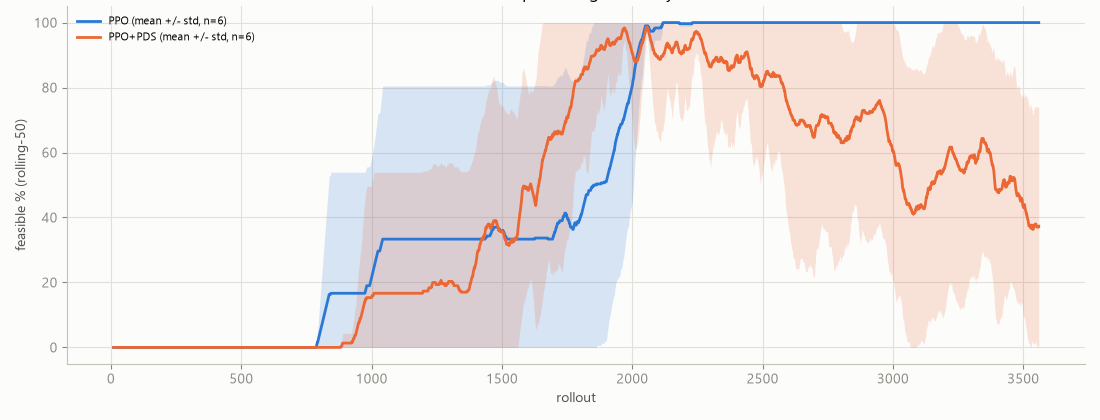
\includegraphics[width=\columnwidth]{figures/fig_rolling_feasible_A.png}\\[1pt]
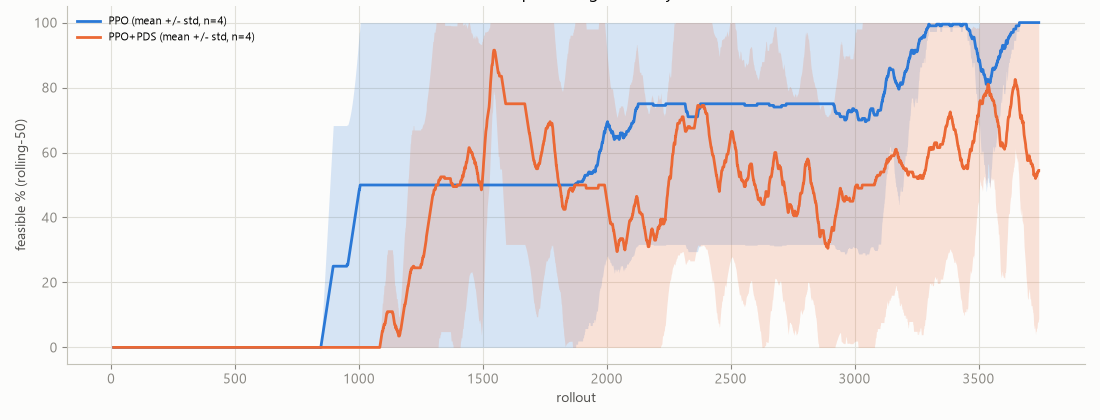
\includegraphics[width=\columnwidth]{figures/fig_rolling_feasible_B.png}
\caption{Held-out feasibility (50-rollout rolling mean; mean $\pm1$ std across seeds) for Budget A (top, 6 seeds) and Budget B (bottom, 4 seeds). PDS-GAE becomes feasible earlier but oscillates; PPO stays at or near 100\% once reached.}
\label{fig:feasible}
\end{figure}

\subsection{Mechanism of the Speed-Up}
On every PDS-GAE rollout we also compute the ordinary TD residual from the same data and critics at no extra cost. In agreement with Proposition~\ref{prop:rb}, $\mathrm{std}(\delta^{\mathrm{pre}})<\mathrm{std}(\delta^{\mathrm{TD}})$ in 80.5\% (A) and 83.0\% (B) of rollouts, with a mean ratio of 0.93. The reduction is concentrated early in training (ratio 0.80 and 0.82 over the first 200 rollouts; 0.93 and 0.94 over the last 500), consistent with Table~\ref{tab:speed}, where the advantage is largest at loose thresholds. The PDS-GAE advantage correlates only weakly with its ordinary-GAE counterfactual (Pearson 0.21, sign agreement 54\%). With learned critics, the PDS residual is therefore a lower-variance estimate of a signal that is only partly the same as the ordinary one.
% Optional figure (re-enable if space permits):
% \begin{figure}[t]\centering
% 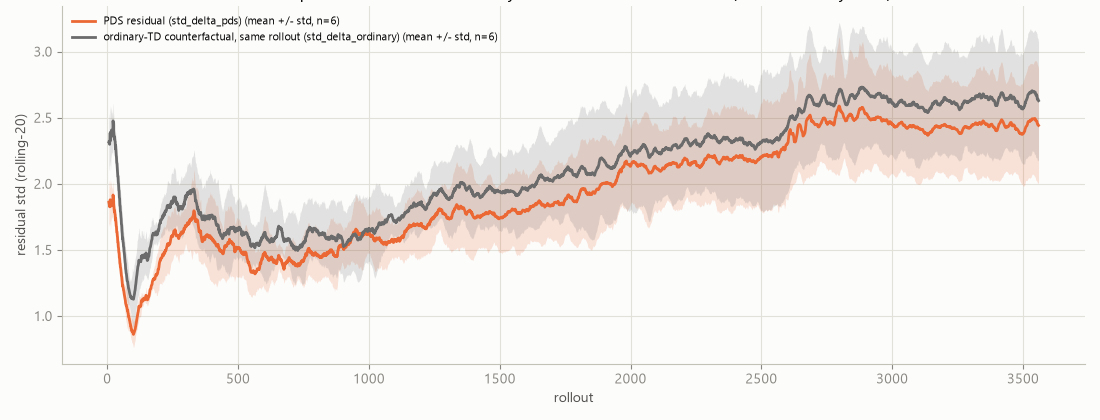
\includegraphics[width=\columnwidth]{figures/fig_residual_variance_A.png}
% \caption{Std of $\delta^{\mathrm{pre}}$ (orange) and of the ordinary TD residual on the same rollouts (grey), Budget A (rolling-20, mean $\pm1$ std, 6 seeds).}
% \label{fig:residual}\end{figure}

\subsection{Final Reliability and Quality}

\begin{table}[t]
\caption{Last 500 Rollouts: Feasibility (Mean [Seed Range]), Budget Use, Quality Among Feasible Rollouts, Policy Entropy}
\label{tab:tail}
\centering
\footnotesize
\setlength{\tabcolsep}{2.4pt}
\begin{tabular}{@{}llcccccc@{}}
\toprule
 & Method & Feasible (\%) & $\frac{J_D}{\bar D}$ & $\frac{J_B}{\bar B}$ & PSNR & $J_Q$ & $\mathcal{H}(\pi)$\\
\midrule
\multirow{2}{*}{A} & PPO     & \textbf{100.0} [100, 100] & 2.7\%  & 91.5\% & 51.95 & 25.61 & 1.38\\
                   & PDS-GAE & 50.0 [0, 96.4]            & 89.6\% & 97.6\% & 51.95 & 25.59 & 2.06\\
\midrule
\multirow{2}{*}{B} & PPO     & \textbf{98.4} [93.6, 100] & 25.6\% & 89.3\% & 51.87 & 25.45 & 1.07\\
                   & PDS-GAE & 68.9 [17.8, 100]          & 62.9\% & 97.4\% & 51.91 & 25.59 & 2.43\\
\bottomrule
\end{tabular}
\end{table}

Over the last 500 rollouts (Table~\ref{tab:tail}), PPO is feasible in 100\% (A) and 98.4\% (B) of held-out evaluations and PDS-GAE in 50.0\% and 68.9\%, with large differences between seeds. Quality among feasible rollouts is practically identical: PSNR differs by at most 0.04\,dB and $J_Q$ by at most 0.14 (about 84\% of its maximum for both), and neither method leads in both budgets. Power is not constrained, and PDS-GAE uses more of it (39.2 vs.\ 30.6\,mW in A; 32.7 vs.\ 28.9\,mW in B; highest level 50\,mW).

\subsection{Why Reliability Lags: Operating at the Boundary}
The Budget-A diagnostics form a consistent chain.
(i)~\emph{Lower, steadier multipliers.} At the end of training, $\mu_D=5.9\pm0.46$ for PDS-GAE vs.\ $11.4\pm1.47$ for PPO and $\mu_B=7.1\pm1.59$ vs.\ $9.1\pm5.67$ (mean $\pm$ across-seed std). This is consistent with PDS-GAE responding to costs sooner, so dual ascent accumulates less, whereas PPO's slower response lets $\mu_D$ overshoot, the integral-control effect analyzed in~\cite{stooke2020pid}.
(ii)~\emph{Boundary operation.} PDS-GAE reaches both budgets quickly and then operates on them (Fig.~\ref{fig:budget}), using 89.6\% of the stall budget; PPO's large $\mu_D$ keeps it at 2.7\%.
(iii)~\emph{Residual stochasticity.} PDS-GAE's final entropy is 1.5$\times$ higher (2.06 vs.\ 1.38), and its mean KL divergence between consecutive policies over the last 500 rollouts is 1.8$\times$ higher (0.024 vs.\ 0.013), so its policy is still changing.
(iv)~\emph{Consequence.} Near the boundary, episode-level fluctuations of a more random policy cross the budget often. The empirical probability of exceeding a margin $\varepsilon$ falls earlier for PDS-GAE but rises again after 2000--3000 rollouts for every $\varepsilon$, whereas PPO's reaches zero after about 2100 rollouts and stays there (Fig.~\ref{fig:convprob}). PDS-GAE's violation therefore does not converge in probability within the trained horizon. Decomposing $v$, PDS-GAE removes the stall term by about 500 rollouts, the remaining violation is tile-driven until about 1600 rollouts, and the stall term then reappears and dominates. On late-training held-out episodes, PDS-GAE stalls in 7.2\% of slots (PPO: 1.3\%) with a median stall of 0.100\,s (PPO: 0.027\,s), and it adds discretionary tiles in 62.4\% of slots (PPO: 50.8\%).
We found no support for overly aggressive actor updates (KL, entropy, and clip fraction were flat across four relapse events) or for a vanishing advantage signal.

\begin{figure}[t]
\centering
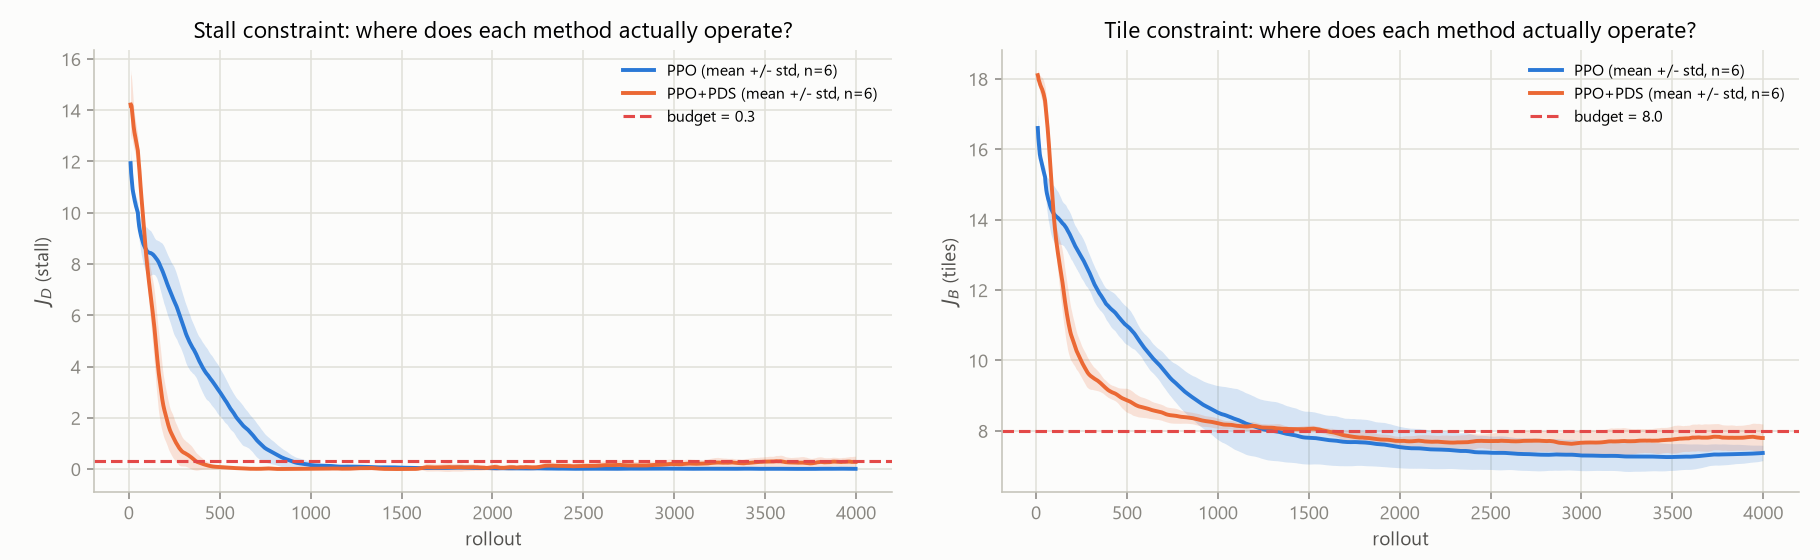
\includegraphics[width=\columnwidth]{figures/fig_budget_trajectories_A.png}
\caption{Held-out stall return $J_D$ (left) and tile return $J_B$ (right), Budget A (mean $\pm1$ std, 6 seeds; dashed: budgets). PDS-GAE reaches both budgets faster and operates at them; PPO settles well inside the stall budget.}
\label{fig:budget}
\end{figure}

\begin{figure}[t]
\centering
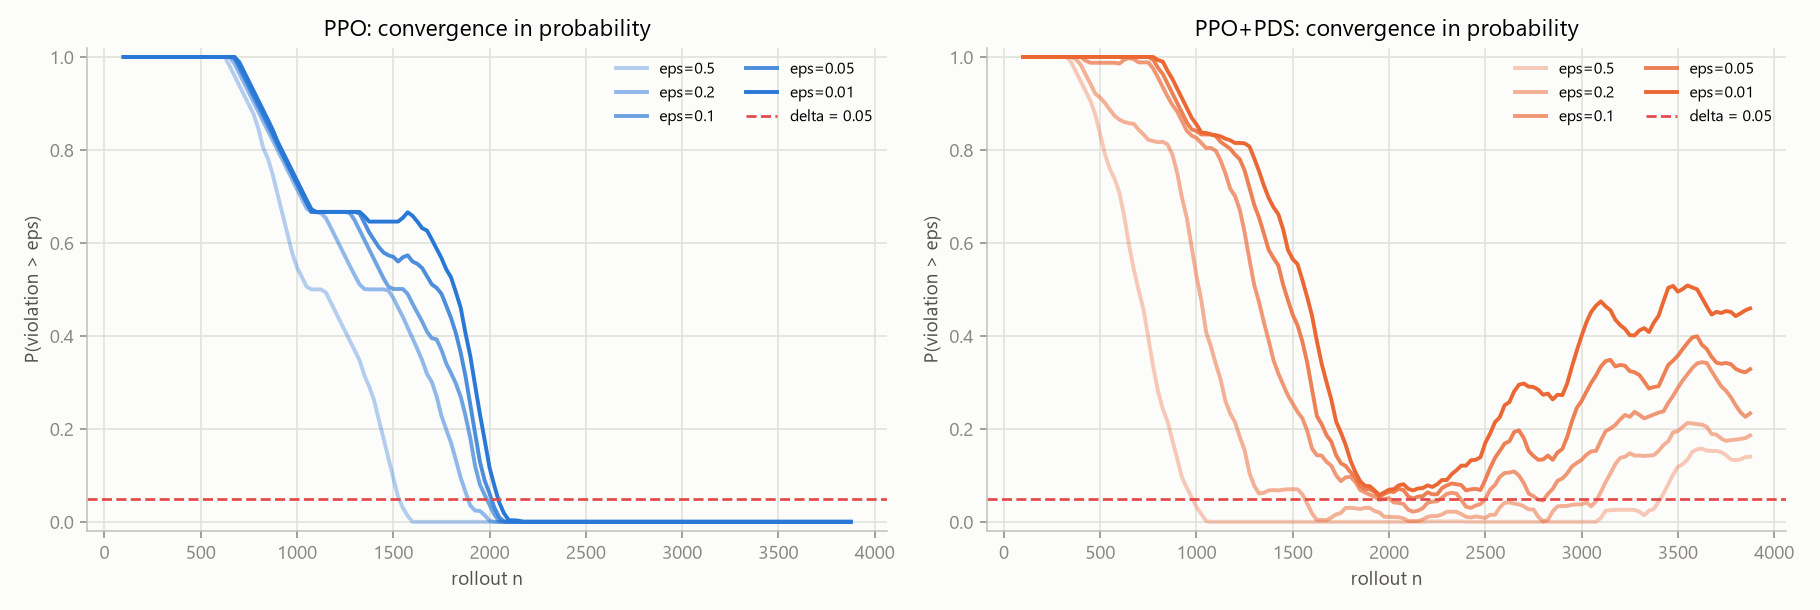
\includegraphics[width=\columnwidth]{figures/fig_conv_in_probability_A.png}
\caption{Empirical probability that the held-out violation exceeds $\varepsilon$ over a sliding window of 200 rollouts $\times$ 6 seeds, Budget A (dashed: $0.05$). PPO (left) reaches zero for every $\varepsilon$; PDS-GAE (right) falls earlier but rises again late in training.}
\label{fig:convprob}
\end{figure}
% Optional figures (re-enable if space permits):
% 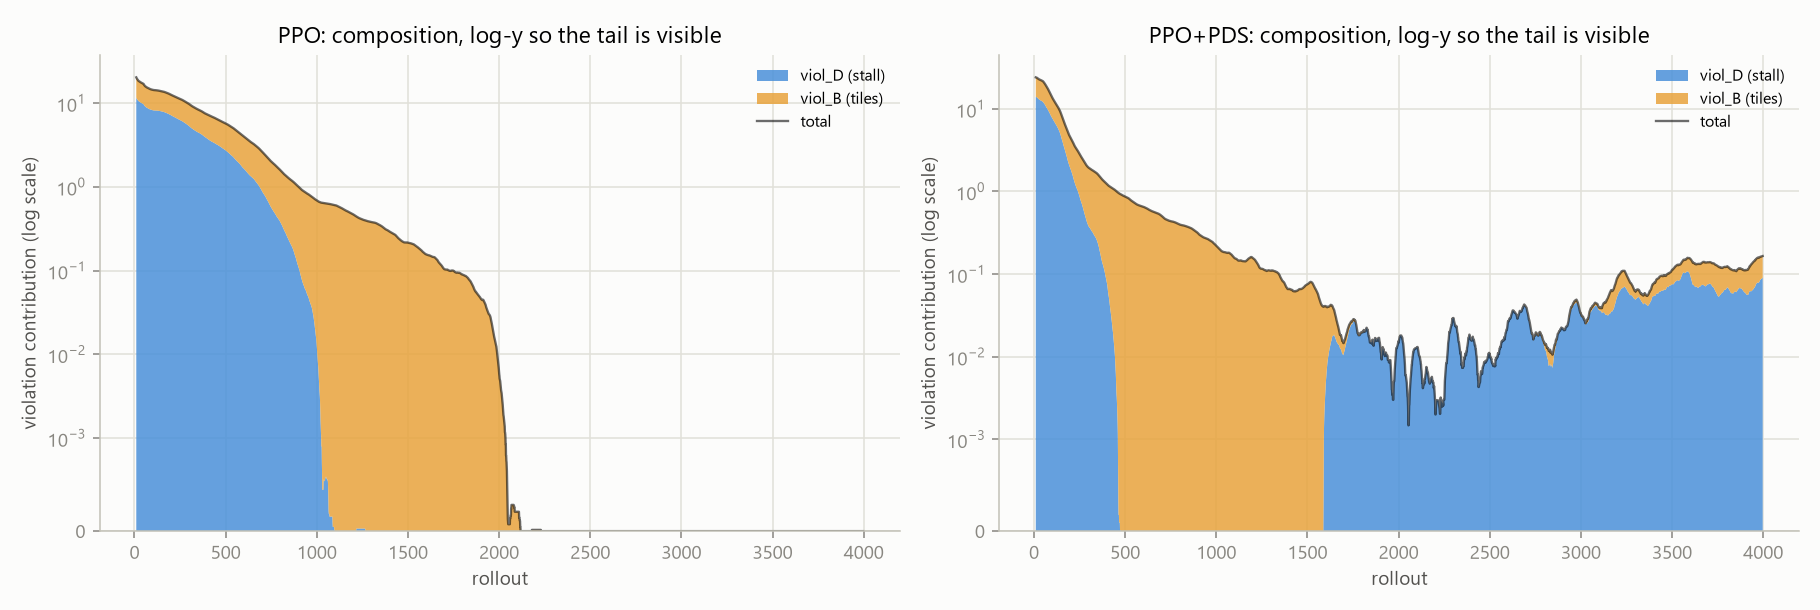
\includegraphics[width=\columnwidth]{figures/fig_violation_composition_A.png}  % stall vs tile violation terms, log scale
% 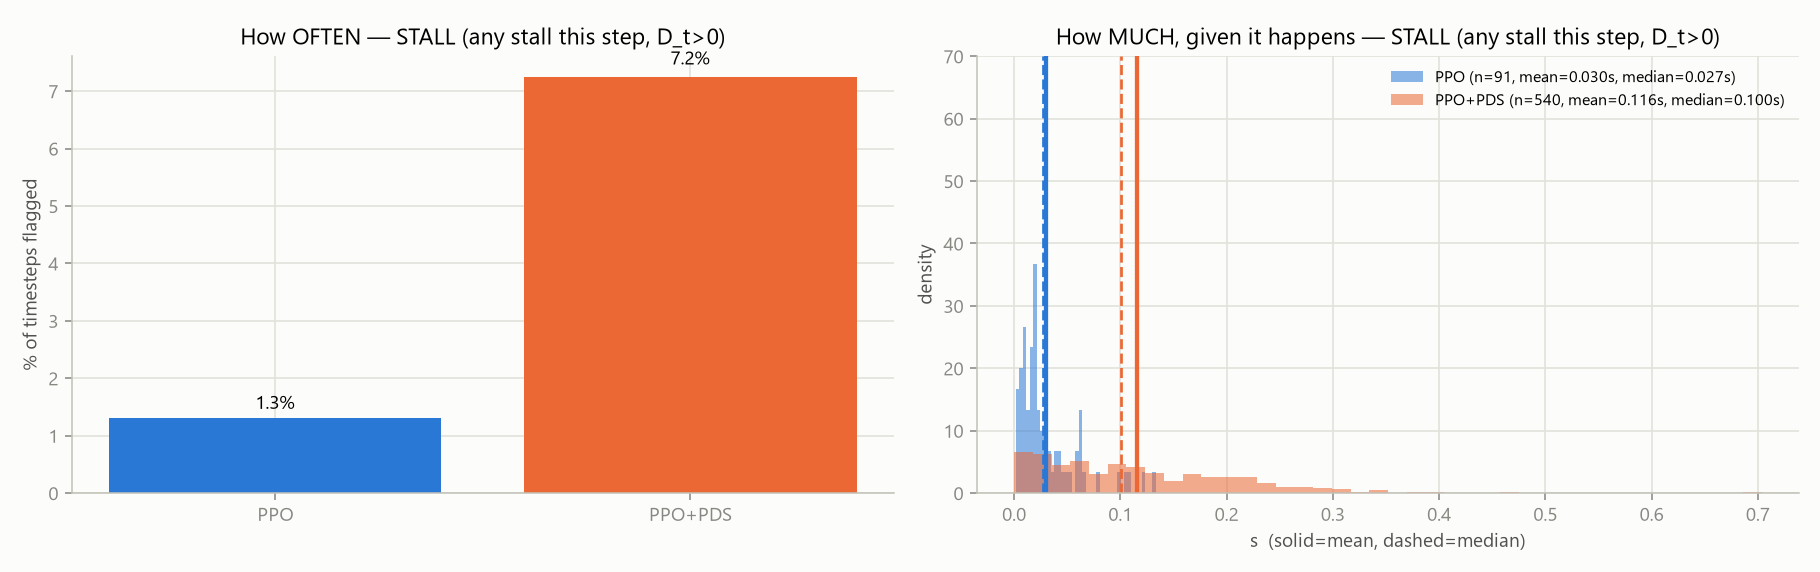
\includegraphics[width=\columnwidth]{figures/fig_instantaneous_stall_A.png}    % per-slot stall frequency and magnitude

\subsection{Virtual Experience}
VE is implemented and was verified: the physics recomputation reproduces the executed transition exactly; a second environment instance stepped with a different action yields the identical viewport and next channel, which confirms (A1); VE sampling leaves the real actions unchanged; and the PDS-critic pass changes no actor or $V_\phi$ parameter. Ten PDS-GAE+VE runs ($\BVE=8$, $T=10$, seeds of Table~\ref{tab:speed}) are in progress and will be compared against Tables~\ref{tab:speed} and~\ref{tab:tail}.
% TODO: replace with VE results once the 10 PDS-GAE+VE arms finish. Compare against a no-VE control produced by the
% CURRENT code (single combined pass when VE is off), not the three early controls launched from commit f6ed9cd.
Because the diagnostics above do not point to a data-starved $\Vt_\psi$, we do not expect VE alone to remove the oscillation.

% =====================================================================
\section{Discussion and Limitations}
\label{sec:discussion}

\textbf{Speed versus reliability.} The two methods fail in opposite directions. PDS-GAE learns the trade-off quickly and uses its budgets almost fully, but it oscillates across the boundary. PPO reaches the boundary slowly and then overshoots into a conservative region at no measurable quality gain. Remedies for PDS-GAE that we have not yet tested include PID-damped dual updates~\cite{stooke2020pid}, state-augmented multipliers~\cite{calvofullana2024state}, a safety margin $\bar b_j-\varepsilon$, and a faster multiplier step.

\textbf{Seed sensitivity.} With seed~4 included in both methods, the loose-threshold speed-ups barely change (A: 2.8$\times$/2.1$\times$ at $v<5$/$v<1$; B: 3.5$\times$/2.4$\times$). At $v=0$, however, the advantage disappears in A (0.97$\times$) and shrinks in B (1.2$\times$), and tail feasibility is 98.5\% vs.\ 57.1\% (A) and 98.7\% vs.\ 57.3\% (B). The strict-threshold comparison therefore rests on few seeds.

\textbf{Rollouts and scope.} Each dual step~\eqref{eq:dual} uses a single-policy Monte Carlo estimate over 48 complete episodes, but the rollout length also sets the dual step frequency and the estimate's variance, and it deserves a dedicated study. Per-episode logging has been added for future runs. Our results use one video, three held-out traces, a static UAV, last-viewport prediction, and 36-slot episodes. Longer episodes, more episodes per rollout, and comparisons with heuristics and with~\cite{chakareski2025mmsp} are future work.

% =====================================================================
\section{Conclusion}
We cast tile-selective aerial 360\textdegree{} streaming as a CMDP with an exact known/random transition split and exploited this split in PPO through a PDS critic propagated by GAE and through policy-sampled virtual experience. PDS-GAE reaches moderate constraint satisfaction 2.1--3.5$\times$ faster and stall feasibility 2.6--3.4$\times$ faster than PPO at equal quality, which is consistent with the lower residual variance predicted by Proposition~\ref{prop:rb}. It does not yet deliver reliable feasibility, because it settles on the constraint boundary. Stabilizing the dual dynamics and evaluating VE are the next steps.

% =====================================================================
% TODO before submission: confirm venue/status of [lu2026resource] and [mohammadhosseini2026stochastic]
% (manuscripts shared by the authors; not found as published items).
\begin{thebibliography}{00}

\bibitem{chakareski2022spm}
J.~Chakareski, M.~Khan, and M.~Yuksel, ``Towards enabling next generation societal virtual reality applications for virtual human teleportation,'' \emph{IEEE Signal Process. Mag.}, vol.~39, no.~5, pp.~22--41, Sep. 2022, \href{https://arxiv.org/abs/2208.04998}{arXiv:2208.04998}.

\bibitem{chakareski2025mmsp}
J.~Chakareski, L.~Wang, and N.~Mastronarde, ``Reinforcement learning-based dynamic resource allocation for aerial 360\textdegree{} video VR streaming,'' in \emph{Proc. IEEE MMSP}, 2025, pp.~328--333, doi: \href{https://doi.org/10.1109/MMSP64401.2025.11324098}{10.1109/MMSP64401.2025.11324098}.

\bibitem{corbillon2017viewport}
X.~Corbillon, G.~Simon, A.~Devlic, and J.~Chakareski, ``Viewport-adaptive navigable 360-degree video delivery,'' in \emph{Proc. IEEE ICC}, May 2017, pp.~1--7.

\bibitem{mohammadhosseini2025asl360}
A.~Mohammadhosseini, J.~Chakareski, and N.~Mastronarde, ``ASL360: AI-enabled adaptive streaming of layered 360\textdegree{} video over UAV-assisted wireless networks,'' in \emph{Proc. IEEE GLOBECOM}, 2025, \href{https://arxiv.org/abs/2509.10544}{arXiv:2509.10544}.

\bibitem{powell2011adp}
W.~B.~Powell, \emph{Approximate Dynamic Programming: Solving the Curses of Dimensionality}, 2nd~ed. Hoboken, NJ, USA: Wiley, 2011.

\bibitem{mastronarde2011fast}
N.~Mastronarde and M.~van der Schaar, ``Fast reinforcement learning for energy-efficient wireless communication,'' \emph{IEEE Trans. Signal Process.}, vol.~59, no.~12, pp.~6262--6266, Dec. 2011, \href{https://arxiv.org/abs/1009.5773}{arXiv:1009.5773}.

\bibitem{sharma2020accelerated}
N.~Sharma, N.~Mastronarde, and J.~Chakareski, ``Accelerated structure-aware reinforcement learning for delay-sensitive energy harvesting wireless sensors,'' \emph{IEEE Trans. Signal Process.}, vol.~68, pp.~1409--1424, 2020. [Online]. Available: \href{https://ieeexplore.ieee.org/document/8998306}{IEEE Xplore}

\bibitem{mastronarde2013joint}
N.~Mastronarde and M.~van der Schaar, ``Joint physical-layer and system-level power management for delay-sensitive wireless communications,'' \emph{IEEE Trans. Mobile Comput.}, vol.~12, no.~4, pp.~694--709, Apr. 2013.

\bibitem{corra2025lowcomplexity}
A.~Corra, N.~Mastronarde, and J.~Chakareski, ``Low-complexity physics-informed reinforcement learning using post-decision states with stochastic sampling,'' in \emph{Proc. IEEE ICC}, 2025, pp.~4559--4564, doi: \href{https://doi.org/10.1109/ICC52391.2025.11161698}{10.1109/ICC52391.2025.11161698}.

\bibitem{mohammadhosseini2026stochastic}
A.~Mohammadhosseini, A.~Corra, M.~Shi, N.~Mastronarde, and J.~Chakareski, ``Physics-informed stochastic post-decision state reinforcement learning for computationally-efficient IoT sensor scheduling,'' manuscript, 2026.

\bibitem{lu2026resource}
Z.~Lu, J.~Chakareski, and N.~Mastronarde, ``Resource-constrained deep post-decision state learning for wireless sensing system scheduling,'' manuscript, 2026.

\bibitem{liu2021partial}
D.~Liu, J.~Zhao, C.~Yang, and L.~Hanzo, ``Accelerating deep reinforcement learning with the aid of partial model: Energy-efficient predictive video streaming,'' \emph{IEEE Trans. Wireless Commun.}, vol.~20, no.~6, pp.~3734--3748, Jun. 2021, \href{https://arxiv.org/abs/2003.09708}{arXiv:2003.09708}.

\bibitem{felizardo2025pdppo}
L.~K.~Felizardo, E.~Fadda, P.~Brandimarte, E.~Del-Moral-Hernandez, and M.~C.~V.~Nascimento, ``A reinforcement learning method for environments with stochastic variables: Post-decision proximal policy optimization with dual critic networks,'' 2025, \href{https://arxiv.org/abs/2504.05150}{arXiv:2504.05150}.

\bibitem{harutyunyan2019hindsight}
A.~Harutyunyan \emph{et al.}, ``Hindsight credit assignment,'' in \emph{Proc. NeurIPS}, 2019, \href{https://arxiv.org/abs/1912.02503}{arXiv:1912.02503}.

\bibitem{altman1999constrained}
E.~Altman, \emph{Constrained Markov Decision Processes}. Boca Raton, FL, USA: CRC Press, 1999.

\bibitem{tessler2019rcpo}
C.~Tessler, D.~J.~Mankowitz, and S.~Mannor, ``Reward constrained policy optimization,'' in \emph{Proc. ICLR}, 2019, \href{https://arxiv.org/abs/1805.11074}{arXiv:1805.11074}.

\bibitem{stooke2020pid}
A.~Stooke, J.~Achiam, and P.~Abbeel, ``Responsive safety in reinforcement learning by PID Lagrangian methods,'' in \emph{Proc. ICML}, 2020, pp.~9133--9143, \href{https://arxiv.org/abs/2007.03964}{arXiv:2007.03964}.

\bibitem{calvofullana2024state}
M.~Calvo-Fullana, S.~Paternain, L.~F.~O.~Chamon, and A.~Ribeiro, ``State augmented constrained reinforcement learning: Overcoming the limitations of learning with rewards,'' \emph{IEEE Trans. Autom. Control}, vol.~69, no.~7, pp.~4275--4290, Jul. 2024, \href{https://arxiv.org/abs/2102.11941}{arXiv:2102.11941}.

\bibitem{schulman2016gae}
J.~Schulman, P.~Moritz, S.~Levine, M.~Jordan, and P.~Abbeel, ``High-dimensional continuous control using generalized advantage estimation,'' in \emph{Proc. ICLR}, 2016, \href{https://arxiv.org/abs/1506.02438}{arXiv:1506.02438}.

\bibitem{schulman2017ppo}
J.~Schulman, F.~Wolski, P.~Dhariwal, A.~Radford, and O.~Klimov, ``Proximal policy optimization algorithms,'' 2017, \href{https://arxiv.org/abs/1707.06347}{arXiv:1707.06347}.

\bibitem{chakareski2021dataset}
J.~Chakareski, R.~Aksu, V.~Swaminathan, and M.~Zink, ``Full UHD 360-degree video dataset and modeling of rate-distortion characteristics and head movement navigation,'' in \emph{Proc. ACM MMSys}, 2021, pp.~267--273, doi: \href{https://doi.org/10.1145/3458305.3478447}{10.1145/3458305.3478447}.

\bibitem{raffin2021sb3}
A.~Raffin, A.~Hill, A.~Gleave, A.~Kanervisto, M.~Ernestus, and N.~Dormann, ``Stable-Baselines3: Reliable reinforcement learning implementations,'' \emph{J. Mach. Learn. Res.}, vol.~22, no.~268, pp.~1--8, 2021. [Online]. Available: \url{https://jmlr.org/papers/v22/20-1364.html}

\end{thebibliography}

\end{document}
